
\section{Teoria de Jogos e Coordenação}
\begin{frame}

\begin{center}
{\huge Capítulo 4 -- Teoria de Jogos e  Coordenação}

3 partes fundamentais:

\begin{enumerate}
  \item Teoria de Jogos
  \item Coordenação
  \item Planejamento (capítulo 5)
\end{enumerate}
Nesta ordem
\end{center}

\end{frame}

%-----------------------------------------------------------


%-----------------------------------------------------------


\section{Estratégias de Jogos}
\begin{frame}

    \frametitle{Teoria de Jogos}
    \begin{itemize}
    \pause
      \item SMA como um comunidade que coopera, \textit{compete},  negocia, etc
      \pause
      \item Asssim é necessária uma métrica 
      entre todos os agentes (\textit{local})
        para levantar um valor \textit{global} de eficiência $\Rightarrow \Rightarrow $ Teoria de Jogos (TJ)
        
        \pause
      \item TJ: uma área a parte que coopera com SMAs
    
    \end{itemize}
\end{frame}


\begin{frame}

    \frametitle{Contextualizando a Teoria de Jogos}
    \begin{itemize}
    \item SMA tem uma visão social $\Rightarrow $ o que seria bom para comunidade toda de agentes?
    
    \item Em TJ, como a decisão \textbf{individual} afeta coletivamente
    \item Estabelecida as regras do jogo (\textit{mecanismo de negociação}),
    qual é a estratégia que seria adotada pelo agente racional?
    
    \item Hoje: TJ via exemplo do \textit{dilema do prisioneiro},
    identificando conceitos tais como: estratégias dominantes, de equilíbrio, equilíbrio de Nash etc.
    
    \end{itemize}
\end{frame}


%-----------------------------------------------------------

\subsection{Teoria de Jogos Aplicado a SMA}

\begin{frame}

\frametitle{Dilema do Prisioneiro}

    
\begin{figure}[!ht]
\centering
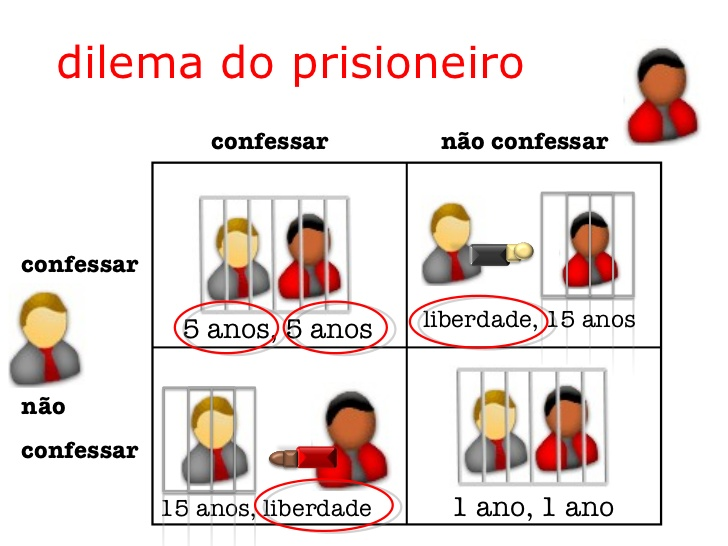
\includegraphics[height =.6\textheight, width=.7\textwidth]{figuras/dilema_prisioneiros01.jpg}
\caption{Memorize a idéia}
%\label{ag_01}
\end{figure}


\end{frame}





\begin{frame}

    \frametitle{Dilema do Prisioneiro}
   
    
\begin{quotation}
        Houve um assassinato e existem dois suspeitos, A e B. Se não se conseguir provar quem foi o assassino, a pena seria de apenas 6 meses por porte de arma.
Se um suspeito acusa (trair ou delatar) o outro e este não se defender (fica calado), então  será condenado a 10 anos. Assim, o traidor que colabora com a polícia sairá livre. Se os dois se acusarem mutuamente a pena é de 5 anos para cada um, pois a
polícia não acredita em nenhum dos dois.
    \end{quotation}
    

   
\end{frame}
    
\begin{frame}

    \frametitle{Dilema do Prisioneiro}
   
\begin{itemize}
  
  \item Como os suspeitos não conhecem a \textit{Teoria dos Jogos}, o normal será que se acusem mutuamente (agentes racionais)
    
  \item Os suspeitos serão interrogados em separado e não tem acesso a(s) resposta(s) do outro

\item Sim, plural: \textit{rodadas} ou \textit{jogadas} de respostas!

\item Muitas \textit{rodadas} leva a pontos como

\begin{itemize}
  \item \textbf{Estratégias puras}: não mudam ao longo do jogo = \textbf{determinísticas}. Exemplo: sempre mover a peça a frente
  
  
  \item Estratégias mistas: mudam ao longo do jogo 
  
  \item Podem olhar a última jogada sua e  de seu adversário
  
  \item Podem olhar o seu histórico de jogadas e  de seu adversário
  
  \item Nestes 3 últimos casos: complexidade $cresce^{\nearrow }$ muito
\end{itemize}


\end{itemize}

   
\end{frame}

%-----------------------------------------------------------

\begin{frame}

    \frametitle{Coletando os Dados: Dilema do Prisioneiro}
    
    
      \begin{center}
        \begin{tabular}{p{2cm} || p{3cm} | p{3cm}} \hline \hline
  & Prisioneiro B nega   &  Prisioneiro B delata   \\ \hline \hline
        Prisioneiro A nega (silêncio ou não-confessa)  &  Ambos condenados a 6 meses  & A é condenado a 10 anos e B é livre   \\ \hline 
         Prisioneiro A delata (acusa ou trai)     & B é condenado a 10 anos e A é livre & Ambos são condenados a 5 anos \\ 
         \hline \hline
        \end{tabular}
      \end{center}

\end{frame}
%-----------------------------------------------------------


\begin{frame}

    \frametitle{Hipóteses: Dilema do Prisioneiro}
    
    
    \begin{itemize}
      \item  Vamos supor que ambos os prisioneiros são completamente egoístas e a sua única meta é reduzir a sua própria estadia na prisão. Como prisioneiros têm duas opções:
      
      \begin{enumerate}
         \item cooperar com o seu cúmplice e permanecerem calados
         \item ou trair o seu cúmplice e confessar que foi o outro (agentes racionais)
       \end{enumerate}   
       
       \begin{itemize}
         \item   O resultado de cada escolha depende da escolha do cúmplice.     
         \item   Infelizmente, um não sabe o que o outro escolheu fazer. 
       
         \item Eis o \textit{impasse}: é um dilema, qual a melhor jogada?
         
       \end{itemize}
       
       \item Inclusive se pudessem falar entre si, não poderiam estar seguros de confiar um no outro (um diria ao outro que era melhor ficarem calados, e depois trairiam o outro)        
       
    \end{itemize}


\end{frame}

%-----------------------------------------------------------

\begin{frame}
    \frametitle{Analisando os fatos:}

%\begin{small}
\begin{quotation}
Se  esperar que o cúmplice escolha cooperar com ele e permanecerem em silêncio, a opção ótima (individualmente) para o primeiro seria confessar, o que significaria que seria libertado imediatamente, enquanto o cúmplice terá que cumprir uma pena de 10 anos. Se espera que seu cúmplice decida confessar, a melhor opção é confessar também, já que ao menos não receberá a pena completa de 10 anos, e apenas terá que esperar 5, tal como o cúmplice. Se ambos decidirem cooperarem entre si e permanecerem em silêncio, ambos serão libertados em apenas 6 meses.
\end{quotation}
%\end{small}


\end{frame}

%-----------------------------------------------------------

\begin{frame}
    \frametitle{Análise: Dilema do Prisioneiro}

   \begin{itemize}
     \item Acusar o outro (confessar que foi o outro)  é uma \textit{estratégia dominante} para ambos os jogadores. Seja qual for a escolha do outro jogador, podem reduzir sempre sua sentença acusando o outro. 
   
  \item Por infelicidade para os prisioneiros, isto conduz a um resultado ruim, no qual ambos acusam seus companheiros e ambos recebem longas condenações. \textcolor{red}{Aqui se encontra o ponto-chave do dilema ou impasse} 
  
  \item O resultado das acusações individuais produz um resultado que não é ótimo no sentido de Pareto; existe uma situação tal que a utilidade de um dos detidos poderia melhorar (ou mesmo a de ambos) sem que isto implique uma piora para o resto. 
  
  \item \textit{Pareto dominante} é quando há soluções muito boas para um ou mais jogadores. Exemplo: acusar o outro é uma resultado interessante!
  
  \item Ou seja, o resultado no qual ambos os detidos não confessam (silêncio) dominam o resultado no qual os dois escolhem confessar.


   \end{itemize}
   
\end{frame}


%-----------------------------------------------------------


\begin{frame}
    \frametitle{Ótimo de Pareto}

 \begin{itemize}
  
 
   \item Perspectiva de interesse ótimo para o grupo (i.é. dois prisioneiros), o resultado correto é que  ambos cooperassem (entre si, ficando calados).   Pois,  isto reduziria o tempo total de pena do grupo a um total de um ano (6 meses para cada um).

   \item  Qualquer outra decisão seria pior para ambos se considerar \textbf{conjuntamente}.

\item Se um jogador tiver uma oportunidade de castigar o outro jogador ao confessar (delatar o outro), então um resultado cooperativo (um vai para prisão apenas?) pode manter-se.

\pause
   
   
\item Neste jogo tem como solução do ponto de vista \textit{Ótimo de Pareto} a estratégia: A e B negam (ficam calados!)

\item Aqui  é o caso de \textit{Pareto dominado}, pois ambos jogadores prefeririam esta solução, as soluções de \textit{Pareto dominante} (agentes racionais $\Rightarrow $ querem o melhor para si!)
     
 \end{itemize}
 
 
\end{frame}
%-----------------------------------------------------------
 
 
\begin{frame}
    \frametitle{John Nash}
 
     
\begin{figure}[!ht]
\centering
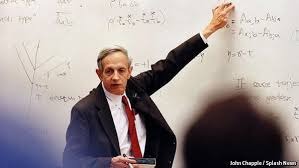
\includegraphics[height =.6\textheight, width=.7\textwidth]{figuras/john_nash01.jpg}
%\caption{Memorize a idéia}
%\label{ag_01}
\end{figure}

\end{frame}
%-----------------------------------------------------------

 
 
\begin{frame}
    \frametitle{Equilíbrio de Nash}

 \begin{itemize}
   
\item Este jogo possui como \textit{Equilíbrio de Nash} de estratégias: 
\textbf{A e B delatam}! Neste caso, o \textit{equilíbrio é dominante}.

\item Porquê é chamado de \textit{Equilíbrio de Nash}?
\pause
 
 \item John Nash: todo jogo tem pelo menos um equilíbrio (mas que não necessariamente domina as estratégias dominantes)
 
\item \textit{Equilíbrio de Nash}: \textit{se a estratégia adotada por A é a melhor dada à estratégia adotada por B e a estratégia adotada por B é a estratégia ótima dada a adotada por A. Ou seja, nenhum dos jogadores pode aumentar seu ganho alterando, de \textbf{forma unilateral}, sua estratégia.}

%%  $u_i(a) \ge u_i(a_{-i}, a^*_i)$
    
  \item   Então o EN é um perfil de uma  ação $a$ tal que $u_i(a) \ge u_i(a_{-i}, a^*_i)$ para cada jogador $i$ e toda ação $a^*$ de $i$
\pause
 
\item No exemplo, assuma que A ou B escolham trair. O que resta para o outro fazer? Trair também! 

\item Ou seja, nenhum dos dois jogadores é benevolentes em sua estratégia (sim, leia-se: jogada)
 %%Apesar disso, se continuarem no seu próprio interesse egoísta, cada um dos dos prisioneiros receberá uma dura pena.
 
% A forma iterada de este jogo (mencionada mais abaixo) oferece uma oportunidade para este tipo de castigo. Nesse jogo, se o cúmplice trai e confessa uma vez, pode-se castigá-lo traindo-o na próxima. Assim, o jogo iterado oferece uma opção de castigo que está ausente no modo clássico do jogo.

 \end{itemize}

\end{frame}
%-----------------------------------------------------------


\begin{frame}
    \frametitle{Formulação: Dilema do Prisioneiro}

\begin{itemize}
  \item $Jogadores = \{A,B\}$
  \item Espaço de estratégia do jogo: $S_A = \{confessa, \:\: nega\}$ e  $S_B = \{confessa, \:\: nega\}$
  \item Espaço do jogo: $S = \{ (nega, nega), (nega,confessa), (confessa, nega), (confessa, confessa) \}$
  \item Função de utilidade: $u_i: S \rightarrow R$ onde $i \in \{A,B\}$
  
  \item No caso $u_A (s): S \rightarrow R$ e $u_B (s): S \rightarrow R$

  \item Assim o mapeamento desta \textbf{função de utilidade} dos jogadores $A$ e $B$:
  
  \begin{itemize}
    \item Para o jogador A:  $u_A (nega, nega) = -1$, $u_A(nega, confessa) = 0$, $u_A(confessa, nega) = -10$  e  $u_A(confessa, confessa) = -5$
  
    \item  Para o jogador B:  $u_B(nega, nega) = -1$, $u_B(nega, confessa) = -10$, $u_B(confessa, nega) = 0$  e  $u_B(confessa, confessa) = -5$
    
  \end{itemize}
  
\end{itemize}


\end{frame}


%-----------------------------------------------------------
\begin{frame}
\frametitle{Construindo uma Matriz de Ganhos:}

\begin{table}[!ht]
  \caption{Função Utilidade}
  \begin{center}
  
    \begin{tabular}{c||c|c}
    \hline \hline
               & B Nega & B Delata  \\     \hline \hline
     A Nega\footnote{Ficar calado.}    &   (-1,-1)     &  (-10, 0)  \\     \hline 
     A Delata\footnote{Trair o outro.}  &    (0, -10)   &  (-5,-5)   \\
         \hline \hline
    \end{tabular}
  \end{center}

  \label{tab_01}

\end{table}


\begin{itemize}
  \item Sendo \textit{egoísta}, a melhor estratégia é delatar seu companheiro e este não se defender
  
  \item Assim, seja qual for a opção do adversário, individualmente, qualquer um se sai melhor traindo ou delatando o outro
  
  \item Ambos chegam individualmente a conclusão \textbf{racional}: \textit{trair}!
  
  \item Nesta lógica individual, as penas somam 10 anos de prisão!
    
  \end{itemize}


\end{frame}

%----------------------------------------------------------

\begin{frame}
\frametitle{Reflexões: Dilema do Prisioneiro}

\begin{itemize}
  \item E se os jogadores aprendessem a \textit{cooperar} após sucessivas jogadas?

  \item Assim suge o \textit{princípio da reciprocidade}, onde o jogador $B$   deve cooperar com $A$ seguindo-o na sua escolha

\pause 
  \item Do livro \textit{A evolução da cooperação: o dilema do prisioneiro e a teoria de jogos} (1984),  de Robert Axelrod, tem-se a terminologia do \textit{ganha-ganha}: 
    
  \begin{center}
    \begin{tabular}{c||p{3cm}|p{3cm}}
    \hline \hline
                & B Coopera & B Delata  \\     \hline \hline
     A Coopera  &   ganha -- ganha     & perda substancial -- ganho substancial  \\     \hline 
     A Delata   &    	ganho substancial -- perda substancial &  	perde -- perde   \\
         \hline \hline

    \end{tabular}
  \end{center}

\end{itemize}

\end{frame}
%----------------------------------------------------------

\begin{frame}
\frametitle{Reflexões: Dilema do Prisioneiro}

\begin{itemize}
\item Outros exemplos: corrida de bicicleta (\textit{Tour de France}, Giro na Itália, etc)  onde há um revezamento na liderança para se poupar, nem se assume a liderança isolada para não se desgastar!

\item O problema da troca de malas

\item \textit{The refund}: recompensa em dizer a verdade 

\item ... ver outros exemplos e TODOS se identificam

\item Como integrar isto a SMAs?
\end{itemize}

\end{frame}

\section{Teoria de Jogos e SMA}


\begin{frame}
\frametitle{Correlação TJ e SMA}

\begin{itemize}
  \item Número de agentes (n): $n > 1$
  \item Cada agente escolhe \textbf{uma estratégia} ou \textbf{uma ação}: $a_i$
  \item Um \textbf{perfil de ações} ou  de \textbf{ações conjuntas} é definido pea tupla de ações individuais: $(a_1, a_2, ...a_n)$
  
     \item Define-se uma ação de todos agentes menos do agente $i$ por: $a_{-1}$
  
  \item Assim uma sequência $(a_i,a_{-1})$ indica que o agente $i$ fez uma ação, e no estado seguinte
  todos  (ou um só, no caso de jogo de adversário) fizeram uma ação conjunta, menos o agente $i$
  
  \item O jogo ocorre em estados  (discretos), com suas recompensas/punições fixas
  
  \item Cada agente tem uma função de avaliação, que indica a \textit{bondade}   ou \textit{intencionalidade} do agente
\end{itemize}

\end{frame}




\begin{frame}
\frametitle{Correlação TJ e SMA}

\begin{itemize}
  \item O estado é observável por todos agentes
  \item Há um \textit{conhecimento comum} e igual por todos agentes
  \item Cada agente ao realizar uma ação $\Leftrightarrow $ jogo de \textbf{\textit{tiro-único}} (visto anteriormente)
  \item Todos agentes escolhem as ações: simultaneamente e individualmente
  \item Nenhum agente é informado sobre o \textbf{{\em tiro}} ou \texttt{\textit{decisão}} assumida pelos demais agentes
  \item Resultado do jogo: \textit{\underline{depende da seleção conjunta de todas as ações}}!
  \item Uma solução de jogo: uma predição de resultado do jogo, assumindo que todos agentes
  são racionais em suas estratégias!
\end{itemize}

\end{frame}



\begin{frame}
\frametitle{Reflexão TJ e coordenação de SMAs}

\begin{itemize}
  \item Antes de coordenação ....
  \item SMA com a parcialidade de observação do mundo (ver figuras da introdução),
  força que agentes racionais interajam entre si!
  \item O que é o \textbf{conhecimento} comum (global) e o individual (local) entre os agentes $\Rightarrow $ comprometimento
  \item \textbf{\textit{Observalidade parcial}} dos agentes $\Rightarrow $ há várias consequencias nas tomadas de decisões dos agentes
  \item Exemplo: n-agentes com \textit{observalidade parcial} em um planejamento 
  de suas ações leva a um problema intratável
  \item Então a \textit{função utilidade} é uma medida ... um ponto de partida!
  
\end{itemize}

\end{frame}

%-----------------------------------------------------

\begin{frame}
\frametitle{OK, vamos jogar!}

 Cara e coroa:

    \begin{center}
      \begin{tabular}{c||c|c}
                 & Cara -- B & Coroa -- B \\ \hline \hline
      Cara -- A   & 1, -1     &  -1, 1      \\ \hline
      Coroa -- A   & -1, 1   & 1, -1         \\ \hline \hline
      \end{tabular}
    \end{center}

\pause 

\begin{itemize}
  \item Tabela de penalidade (\textit{pay-off}) de um jogo \textbf{estritamente competitivo} ou \textbf{soma-zero}
 \item Pois $u_1(a) + u_2(a) = 0$
\end{itemize}

\end{frame}

%----------------------------------------------------------

\begin{frame}
\frametitle{OK, vamos jogar!}



 Dois carros (motorista A e motorista B) em um cruzamento, querem cruzar \textit{logo}:

    \begin{center}
      \begin{tabular}{c||c|c}
                 & Avance -- B & Pare -- B \\ \hline \hline
      Avance -- A   & -1, -1     &  1, 0      \\ \hline
      Pare -- A     & 0, 1   & 0, 0         \\ \hline \hline
      \end{tabular}
    \end{center}
    
\pause 
\begin{itemize}
  \item Tabela de penalidade (\textit{pay-off}) para um jogo típico de \textbf{coordenação}. 
  
  \item Pois
se os dois carros desejarem avançar teremos: $u_1(a) + u_2(a) = -2$, consequentemente
uma batida.

\end{itemize}

\end{frame}

%----------------------------------------------------------

\begin{frame}
\frametitle{Exercícios}

\begin{enumerate}
  \item Construa a função de utilidade para jogo \textbf{pedra--papel--tesoura} para este se torne um jogo competitivo. Justifique suas escolhas:
  
    \begin{center}
      \begin{tabular}{l||c|c|c}
                 & Pedra -- B & Papel -- B & Tesoura -- B \\ \hline \hline
      Pedra -- A     &       &     &   \\ \hline
      Papel -- A     &       &       &   \\ \hline
      Tesoura -- A   &       &       &   \\ \hline \hline
      \end{tabular}
    \end{center}


\item Nos 3 últimos exemplos identifique os elementos e os justifique:
\begin{enumerate}
    \item O que é uma estratégia em cada jogo
    \item Há um Pareto dominante?
    \item Qual é o Pareto ótimo?
    \item Onde está o equilíbrio de Nash? (pode haver mais de um)
  \end{enumerate}  
  
\end{enumerate}

\end{frame}

%----------------------------------------------------------




%%% longe


\section{Coordenação}


\begin{frame}
\frametitle{Coordenação}
\begin{itemize}
  \item Um tema amplo em SMA ...
  \item Coordenação $\approx $ a não obstrução entre os agentes 
  \item ou decisões individuais dos agentes que possam levar
  há uma boa decisão conjunta do grupo
\end{itemize}


\end{frame}


%-----------------------------------------------------------

\begin{frame}
\frametitle{Coordenação}
\begin{itemize}
  \item Ainda ... a medida usando a TJ é o equlíbrio de Nash
  \item Exemplo: o exemplo dos carros no cruzamento, tem DOIS (pontos) de equlíbrio de Nash
  \item Neste caso: $u_A(para,avanca) = u_B(avanca, para)$
  \pause
  \item Neste sentido, em que todos agentes $n$ compartilham a mesma função de utilidade, eles serão colaborativos se:
  $u_1(\overrightarrow{acoes}) = u_2\overrightarrow{(acoes}) = \ldots \ldots  u_n(\overrightarrow{acoes})$
  
  \item A notação acima é uma simplificação de: 
  $u_i(a_i, \overrightarrow{a_{-i}})$ 
  
  \end{itemize}


\end{frame}

%-----------------------------------------------------------

\begin{frame}
\frametitle{Abordagens para  Coordenação}
 
 Estruturando o tema de \textit{coordenação}, o mesmo
 discutido segundo suas estratégias:

 \begin{enumerate}
   \item Jogos de Coordenação (fundamentação no capítulo anterior)
   \item Convenções (função) Sociais
   \item Papéis
   \item Grafos de Coordenação, subdivide-se em:
        \begin{enumerate}
          \item Coordenação por Eliminação de Variável
          \item Coordenação por Troca de Mensagem
        \end{enumerate}
   
   
 \end{enumerate}




\end{frame}



%-----------------------------------------------------------


\subsection{Jogos de Coordenação}

\begin{frame}
\frametitle{Jogos de Coordenação}

\begin{itemize}
  \item Exemplo de um casal $\{Abel, Beatriz\}$ que gostam de dançar
    \begin{center}
      \begin{tabular}{c || c | c}
                 & Decansar -- B & Dansar -- B \\ \hline  \hline
      Decansar -- A   & 1, 1     &  0, 0      \\ \hline
      Dansar -- A     & 0, 0     &  1, 1         \\ \hline
      \end{tabular}
    \end{center}

novamente, tem-se dois equilíbrios de Nash e ótimos de Pareto

\item Generalizando estes 2 exemplos (o outro era dos carros no cruzamento), 
define-se formalmente  \textbf{coordenação}
 
 \item \textbf{Coordenação:} \textit{é um processo no qual  um grupo de agentes escolhe um Pareto ótimo e um equílibrio de Nash no jogo}
 
 \item Compartilham a mesma função utilidade
  (\textit{payoff function} -- fugiu a tradução de penalidade), logo, eles  serão
  colaborativos!
 
  \item Vale ressaltar que nesta abordagem os agentes compartilham a mesma função de utilidade $\Rightarrow $ veja tabelas dos exemplos
  
 
\end{itemize}
\end{frame}

%---------------------------------------






%-----------------------------------------------------------
\subsection{Convenção Social}

\begin{frame}%[allowframebreaks=0.9]
\frametitle{Convenção Social}

\begin{itemize}
  \item Como escolher a ação?
  \item Infelizmente, não há tal receita que conduza ao Equilíbrio de Nash (EN)!
  \item Assim receitas devem ser passadas aos agentes visando o EN

\pause
  \item Convenção social (ou lei social): é uma \textit{receita} que visa
  restringir as ações  dos agentes.
  
  \item Assim, os agentes seriam \textit{conduzidos} a terem um comportamento
  social, visando um EN!
  
  \item Que \textit{receitas} seriam estas? Exemplos:
  \pause
  \begin{enumerate}
    \item Agente \textbf{A} escolhe depois de \textbf{B} (afinal no par, \textbf{B} é a Beatriz)
    \item A agente \textbf{B} é animada, sempre quer dançar!
  \end{enumerate}
  
\item A partir disto, o EN é investigado dado os $n$ agentes da comunidade


  \item Sob esta Convenção Social (CS) o conhecimento é comum e nenhum agente pode se
  beneficiar disto para sempre!
 
\end{itemize}


\end{frame}
%-----------------------------------------------------------


\begin{frame}%[allowframebreaks=0.9]
\frametitle{Convenção Social -- Comentários}

\begin{itemize}
  \item Coordenação que usam CS podem se fazer uso de ordenamento dos agentes -- fácil de implementar
  
  \item O agente $i$ faz uma divulgação (\textit{broadcasting}) de sua ação aos $n-1$ agentes, e espera   que todos os  $n-1$ agentes tenham selecionados suas ações
  
  \item Após os $n-1$ agentes tenham decididos suas ações, o agente $i$
  vai escolher a ação que tenha o maior equilíbrio do sistema
  
  \item Note que há um ordenamento fixo entre os agentes com comunicações via  primitivas, de modo que tudo seja uma ordem sincronizada sequencialmente de ações
  
  \item Casos clássicos de \textit{deadlocks} de BD, nem pensar!
  
\end{itemize}

\end{frame}



%%%%--------------------------------------------------------------------
%-----------------------------------------------------------

\subsection{Papel Social}

\begin{frame} %[allowframebreaks=0.9]
\frametitle{Papel Social}

\begin{itemize}
  \item No caso anterior, \textbf{convenção social}, considera-se que um agente pode calcular 
  todo EN antes de fazer uma escolha.
  \item Sim, calcular tudo antes de agir, pode ser muito dispendioso para uma comunidade
com um número  muito elevado de agentes
   \item Então \textbf{reduzir} este número de possíveis ações antes de escolher/selecionar uma ação 
   \item Sim, esta redução implica em velocidade, etc



\end{itemize}

\end{frame}


%-----------------------------------------------------------------
\begin{frame}
\frametitle{Papel Social}

\begin{itemize}
  \item Esta redução do número de um conjunto de ações é pela atribuição de \textbf{papéis sociais}
  \item Logo, esta  atribuição de um papel ao agente em um dado estado, deve inibir os demais agentes
  de agirem como tal
  \item Exemplo: futebol de robô. Um agente de papel na defesa, não jogará no  papel de ataque. 
  
  \item A proposta é que o jogo, terá a sua tarefa de coordenação reduzida, devido o agente atuar em um papel de um \textit{sub-jogo} (\textit{subgame})
  
  \item Logo o equilíbrio será mais fácil de encontrar

\end{itemize}

\end{frame}

%-----------------------------------------------------------------
\begin{frame}%[allowframebreaks=0.9]
\frametitle{Esquema Básico dos Papéis Sociais}


\begin{enumerate}
  \item There is a fixed ordering \{1, 2, . . . , n\} of the roles. Role 1 must be assigned first, followed by role 2, etc.
  
\item  For each role there is a function that assigns to each agent a '\textit{potential}' that reflects how appropriate (uma maximização) that agent is for the specific role, given the current state. For example, the
potential of a soccer robot for the role attacker can be given by its negative Euclidean distance to the ball.

\item  Each agent can be assigned only one role. 

\item Resumindo: ambiente observável, os papéis podem ser repetidos, e variam a cada estado

\end{enumerate}

\end{frame}

%-----------------------------------------------------------------
\begin{frame}% [allowframebreaks=0.9]
\frametitle{Resumindo a coordenação via \textit{papéis sociais}}

\begin{itemize}
  \item O papel 1 é definido para o agente de mais alta habilidade (max)

  \item O algoritmo não é paralelo, é sequencial (começa pelo  agente $i$
  mais hábil no papel $j$)

  \item Todos $i$ agentes, em paralelo, tiveram conhecimento dos $j$ papéis disponíveis (alguns repetidos ou não)

  \item A divulgação dos papéis em geral é transmitida via
\textit{broadcasting}

 \item Um algoritmo guloso na atribuição dos papéis pode ser utilizado 
quando uma comunicação entre agentes está disponível
  
\end{itemize}


\end{frame}

%-----------------------------------------------------------
\subsection{Grafos de Coordenação}

\begin{frame}
\frametitle{Grafos de Coordenação}

pag 26


\begin{huge}

\textbf{ \textcolor{red}{Falta terminar}}
 

\end{huge}
\end{frame}
%-----------------------------------------------------------


\subsubsection{Coordenação por Eliminação de Variáveis}

\begin{frame}
\frametitle{Coordenação por Eliminação de Variáveis}

pag 28


\end{frame}
%-----------------------------------------------------------


\subsubsection{Coordenação por Troca de Mensagens}

\begin{frame}
\frametitle{Coordenação por Troca de Mensagens}

pag 28


\end{frame}
%-----------------------------------------------------------

%-----------------------------------------------------------

%-----------------------------------------------------


\subsection{Exemplos de Coordenação SMAs}

\begin{frame}
\frametitle{Exemplo de Coordenação SMAs}

\begin{figure}[!ht]
\centering
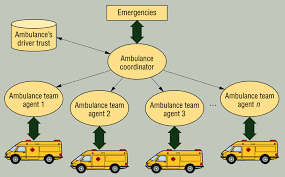
\includegraphics[height =.6\textheight,width=.7\textwidth]{figuras/coordenacao_agentes01.png}
\caption{Coordenação de agentes $\equiv $   SMA}
%\label{ag_01}
\end{figure}
 \end{frame}

%-----------------------------------------------------------

\begin{frame}
\frametitle{Exemplo de Coordenação SMAs}

\begin{figure}[!ht]
\centering
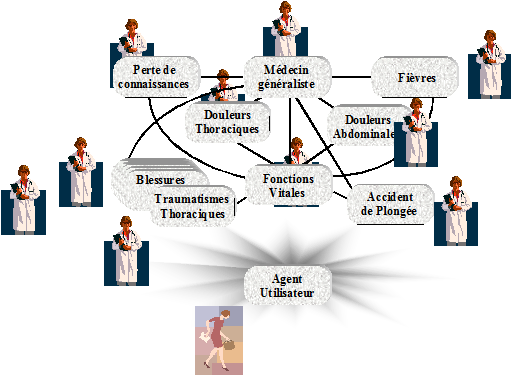
\includegraphics[height =.6\textheight,width=.7\textwidth]{figuras/coordenacao_agentes02.png}
\caption{Coordenação de agentes $\equiv $   SMA}
%\label{ag_01}
\end{figure}
 
\end{frame}


%-----------------------------------------------------------
